\documentclass[titlepage]{article}
\usepackage[utf8]{inputenc}
\usepackage{amsmath, amssymb}

% package for drawing
\usepackage{tikz}
\usepackage{tikz-qtree}
\usetikzlibrary{shapes.geometric}
\usetikzlibrary{positioning}
\usepackage{xcolor}
\usepackage{caption, subcaption}

\newtheorem{theorem}{Theorem}

% Page formatting
\usepackage{geometry}[left = 1, right = 1, top = 1, bottom = 1] % 1 inch page margins

%%% tikz formatting
\definecolor{pruned}{gray}{0.65}
% nodes
\tikzset{
    treenode/.style={align=center, draw=black, thick},
    node_max/.style={treenode, regular polygon, regular polygon sides=3},
    node_min/.style={treenode, regular polygon, regular polygon sides=3, shape border rotate=180},
    node_leaf/.style={draw=black, thin, rectangle, font=\tiny}
}
% alpha-beta label "MACRO"
%\newcommand{\ablab}[2]{
%    label=above:{\scriptsize{\textbf{[#1,#2]}}}
%    }
% not working... yet
% edges
\tikzset{edge from parent/.append style={thin, draw=black}}
%\newcommand{\prunededge}{\edge[dashed, draw=pruned]}
\tikzset{level 1/.style={level distance=56pt, sibling distance=4pt}}
\tikzset{level 2/.style={level distance=64pt, sibling distance=4pt}}
\tikzset{level 3/.style={level distance=64pt, sibling distance=2pt}}

\title{\textbf{Problem Set 2}}
\author{
    Zain Ali (zaa23)\\
    Michael Saunders (mbs189)\\
}
\date{Rutgers University\\Intro. to A.I. - CS440\\Summer 2020}

\begin{document}
\maketitle

\section*{Problem 1}
\begin{figure}[h!]
\centering
\label{minmaxtree}
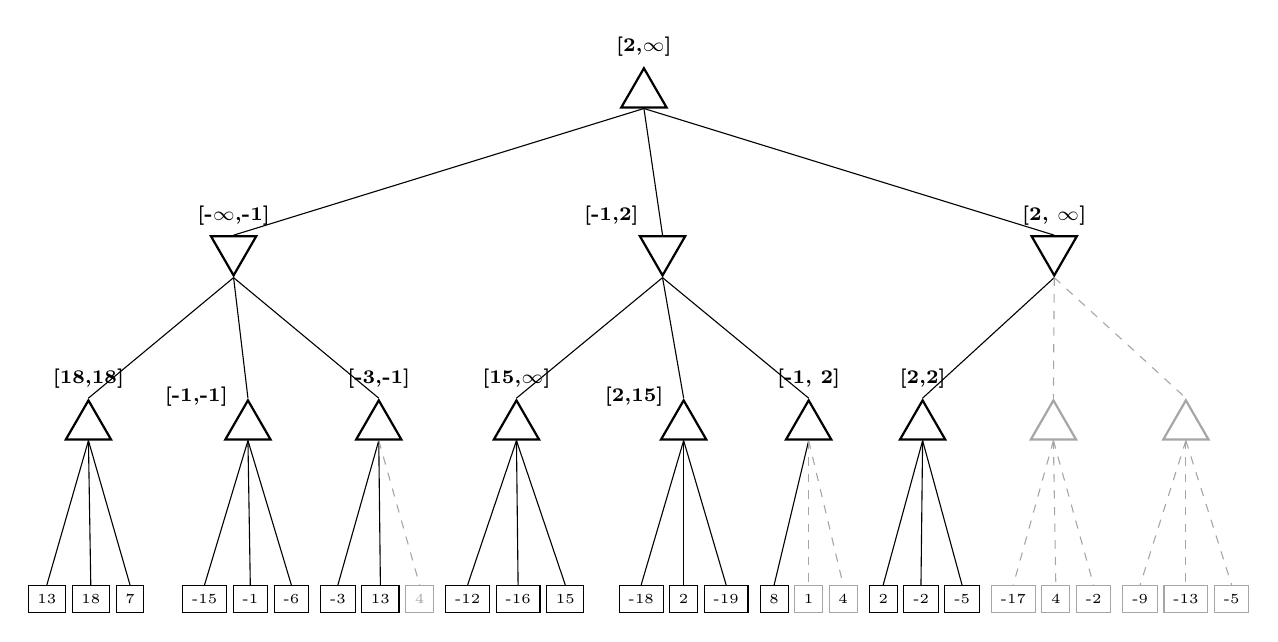
\begin{tikzpicture}[]
    \Tree 
        [.\node[node_max, label=above:{\scriptsize\textbf{[2,\(\infty\)]}}](root){};
            [.\node[node_min, label=above:{\scriptsize\textbf{[-\(\infty\),-1]}}](l1a){};
                [.\node[node_max, label=above:{\scriptsize\textbf{[18,18]}}](l2aa){};
                    [.\node[node_leaf](l3aaa){13};]
                    [.\node[node_leaf](l3aab){18};]
                    [.\node[node_leaf](l3aac){7};]
                ]
                [.\node[node_max, label=above left:{\scriptsize\textbf{[-1,-1]}}](l2ab){};
                    [.\node[node_leaf](l3aba){-15};]
                    [.\node[node_leaf](l3abb){-1};]
                    [.\node[node_leaf](l3abc){-6};]
                ]
                [.\node[node_max, label=above:{\scriptsize\textbf{[-3,-1]}}](l2ac){};
                    [.\node[node_leaf](l3aca){-3};]
                    [.\node[node_leaf](l3acb){13};]
                    \edge[dashed, draw=pruned];[.\node[node_leaf, draw=pruned, text=pruned](l3acc){4};]
                ]
            ]
            [.\node[node_min, label=above left:{\scriptsize\textbf{[-1,2]}}](l1b){};
                [.\node[node_max, label=above:{\scriptsize\textbf{[15,\(\infty\)]}}](l2ba){};
                    [.\node[node_leaf](l3baa){-12};]
                    [.\node[node_leaf](l3bab){-16};]
                    [.\node[node_leaf](l3bac){15};]
                ]
                [.\node[node_max, label=above left:{\scriptsize\textbf{[2,15]}}](l2bb){};
                    [.\node[node_leaf](l3bba){-18};]
                    [.\node[node_leaf](l3bbb){2};]
                    [.\node[node_leaf](l3bbc){-19};]
                ]
                [.\node[node_max, label=above:{\scriptsize\textbf{[-1, 2]}}](l2bc){};
                    [.\node[node_leaf](l3bca){8};]
                    \edge[dashed, draw=pruned];[.\node[node_leaf, draw=pruned](l3bcb){1};]
                    \edge[dashed, draw=pruned];[.\node[node_leaf, draw=pruned](l3bcc){4};]
                ]
            ]
            [.\node[node_min, label=above:{\scriptsize\textbf{[2, \(\infty\)]}}](l1c){};
                [.\node[node_max, label=above:{\scriptsize\textbf{[2,2]}}](l2ca){};
                    [.\node[node_leaf](l3caa){2};]
                    [.\node[node_leaf](l3cab){-2};]
                    [.\node[node_leaf](l3cac){-5};]
                ]
                \edge[dashed, draw=pruned];[.\node[node_max, draw=pruned](l2cb){};
                   \edge[dashed, draw=pruned];[.\node[node_leaf, draw=pruned](l3cba){-17};]
                    \edge[dashed, draw=pruned];[.\node[node_leaf, draw=pruned](l3cbb){4};]
                    \edge[dashed, draw=pruned];[.\node[node_leaf, draw=pruned](l3cbc){-2};]
                ]
                \edge[dashed, draw=pruned];[.\node[node_max, draw=pruned](l2cc){};
                    \edge[dashed, draw=pruned];[.\node[node_leaf, draw=pruned](l3cca){-9};]
                    \edge[dashed, draw=pruned];[.\node[node_leaf, draw=pruned](l3ccb){-13};]
                    \edge[dashed, draw=pruned];[.\node[node_leaf, draw=pruned](l3ccc){-5};]
                ]
            ]
        ]
\end{tikzpicture}
\caption{MIN-MAX Search Tree with Alpha-Beta Pruning.}
\end{figure}

\section*{Problem 2}
To find the probability of a person having Lyme disease given a positive test ($P(A|B)$) we must first define the following:\\
\\
$A$ = has Lyme disease\\
$B$ = positive test\\
$P(A)$ = probability of having Lyme disease = 0.008\\
$P(\neg{A})$ = probability of not having Lyme disease = $1 - P(A)$ = 0.992 \\
$P(B|A)$ = probability of a positive test given the person has Lyme disease = 0.93\\
$P(B|\neg{A})$ = probability of a positive test given the person does not have Lyme disease = 0.16\\
\\
To solve this we will use Bayes's Rule\\
\begin{theorem}[Bayes's Rule]
\[ P(A|B) = \frac{P(B|A) * P(A)}{P(B)} \]
\[ P(A|B) = \frac{P(B|A)*P(A)}{P(B|A)*P(A)+P(B|\neg{A})*P(\neg{A})}\]
\end{theorem}
Using Bayes's Rule:\\

\[ P(A|B) = \frac{0.93*0.008}{0.93*0.008+0.16*0.992}\]
\\
\[ P(A|B) = \frac{0.00744}{0.00744+0.15872}\]
\\
\[ P(A|B) = 0.04477611 = 4.477611\%\]
\\
According to Bayes's Rule, the probability of a person taking a test and finding out they have Lyme disease due to a positive test $(P(A|B))$ is 4.477611\%.

\section*{Problem 3}
Suppose there are 5 balls with distinct colors (blue, yellow, read, green, and pink) in a box. Each time I randomly pick a ball, I record the color of the ball I picked then put it back. I repeat this behavior several times.\\
\\
\textbf{(a) What is the expected number of picking attempts it takes so as to see all colors of balls?}\\
\\
Assuming X is the number of picking attempted it takes to see all colors of balls we will find $E[X]$ using linearity of expectation and expected attempts.\\

\[\text{Golden Rule 1: } E[X] = E[X_1+X_2] = E[X_1] + E[X_2]\]

\[\text{Golden Rule 2: } E[X_i] = \frac{1}{P(X_i)}\]

\[P(X_i) = \text{Probability to pick an i'th unique color}\]\\
The probability for the first unique color is $P(X_1)=1$, the next color probability would be $P(X_2) = \frac{4}{5}$ followed by $P(X_3) = \frac{3}{5}$, $ P(X_4)=\frac{2}{5}$, and $P(X_5)=\frac{1}{5}$. Using that, we can find out how many picks you would need for to get all 5 ball colors.\\

\[E[X] = \sum_{i=1}^{5}E[X_i]=\sum_{i=1}^{5}\frac{1}{P(X_i)}\]\\
\[\sum_{i=1}^{5}\frac{1}{P(X_i)} = \frac{1}{1}+\frac{1}{(\frac{4}{5})}+\frac{1}{(\frac{3}{4})}+\frac{1}{(\frac{2}{5})}+\frac{1}{(\frac{1}{5})}=11\frac{5}{12} \approx 11.42\text{ attempts}\] \\

It is expected to take about 11.42 attempts of picking the colored balls to see every color.\\



\noindent\textbf{(b) If I repeat the picking behavior 6 times, what is the expected number of distinct colors I will see?}\\
\\
Let $X$ = the number of distinct colors recorded after 6 repetitions of picking a ball, recording the color, and replacing the ball.\\
\\
Define Random Variables $x_i$ for $1 \leq i \leq 5$ such that:\\
    \[x_i = 1 \mbox{ if color $i$ was selected at least once, otherwise $x_i = 0$.}\]
The number of distinct colors recorded is the sum of the Random Variables, $x_i$:
    \[X = x_1 + x_2 + x_3 + x_5 + x_5\]
The expected number of distinct colors $E(X)$ is defined as such:\\
    \[E[X] = E[x_1 + x_2 + x_3 + x_4 + x_5].\]
By \emph{linearity of expectation} (golden rule 1),
    \[E[X] = E[x_1] + E[x_2] + E[x_3] + E[x_4] + E[x_5]\]
Since the value of our random variables $x_i$ can only be either $1$ or $0$, we can derive the following:
    \[E[x_i] = 0 * P(x_i = 0) + 1 * P(x_i = 1)\]
    \[E[x_i] = P(x_i = 1)\]
    \[\implies E[X] = \sum_{i=1}^{5}P(x_i = 1)\]
To find $E[X]$ we now just need to find the probability of each random variable $x_i$ having the value of 1.
    \[P(x_i = 1) = P(\mbox{color $i$ is recorded at least once})\]
    \[P(x_i = 1) = 1 - P(\mbox{color $i$ is never recorded})\]
Since we are replacing the balls we choose each time after their color is recorded, then selecting from the same set of 5 colored balls each time, \emph{each color has the same probability of never being chosen.} So, we can simplify the equation further by factoring out a $5$.
        \[E[X] = 5 * P(x_i = 1)\]
        \[E[X] = 5 * (1 - (\frac{4}{5})^6) \approx 3.69 \text{ colors}\]
The expected number of distinct colors recorded after 6 repetitions of the behavior is approximately 3.69.
\end{document}
